\chapter{Programmazione Lineare Mista}

\section{Rifornimento d'Acqua}

\paragraph{Consegna}

Una catena di ristoranti ha stipulato un contratto commerciale con un'industria di acque minerali per la fornitura esclusiva di bottiglie d’acqua. L'industria ha a disposizione quattro impianti di S1, S2, S3, S4 con cui dovrà rifornire i tre ristoranti R1, R2 e R3 della catena. Vista la differente distanza tra gli impianti e i ristoranti e i differenti mezzi di trasporto utilizzati, i costi di trasporto euro/bottiglia di acqua da un impianto ad un bar risultano differenti e sono riassunti nella tabella a lato. Sapendo che:

\begin{itemize}
    \item gli impianti producono giornalmente 125, 150, 130 e 110 bottiglie;
    \item i tre ristoranti necessitano di 160, 175, 180 bottiglie
\end{itemize}

\begin{center}
    \begin{tabular}{||c | c | c | c||}
        \hline
        & R1 & R2 & R3 \\
        \hline
        S1 & 0.4 & 0.3 & 0.2 \\
        \hline
        S2 & 0.2 & 0.3 & 0.5 \\
        \hline
        S3 & 0.1 & 0.6 & 0.2 \\
        \hline
        S4 & 0.5 & 0.1 & 0.3 \\
        \hline
    \end{tabular}
\end{center}

Elaborare un modello di Programmazione Lineare che minimizzi i costi totali di trasporto.

\paragraph{Svolgimento}

Sia $c_{ij}$ il costo del trasporto tra il i-esimo stabilimento e il j-esimo ristorante.
Sia $q_{ij}$ la quantita' di acqua trasportata tra il i-esimo stabilimento e il j-esimo ristorante.
Sia $p_i$ la quantita' di acqua prodotta dall'i-esimo stabilimento.
Sia $a_j$ la quantita' di acqua accolta dal j-esimo ristorante.

\begin{align*}
    min Z &= \Sigma ^{4} _{i=1} \Sigma ^{3} _{j=1} c_{ij} q_{ij} \\
    \Sigma ^{4} _{i=1} q_{ij} &= a_j &\forall j\\
    \Sigma ^{3} _{j=1} q_{ij} &= p_i &\forall i\\
    q_{ij} &\geq 0 &\forall i,j 
\end{align*}

\section{Rifornimento d'Acqua 2.0}

Riprendiamo il problema dell’ ESERCIZIO 1. Supponiamo ora che l’industria voglia che ciascun impianto si prenda carico di almeno il 15\% delle spedizioni e che il costo di trasporto generato dall’impianto S1 sia al massimo 1/4 del costo totale. Come possiamo formulare questi vincoli aggiuntivi? Quale altra modifica al modello precedente è necessario imporre?

\begin{itemize}
    \item gli impianti producono giornalmente 125, 150, 130 e 110 bottiglie;
    \item i tre ristoranti necessitano di 160, 175, 180 bottiglie
\end{itemize}

\begin{center}
    \begin{tabular}{||c | c | c | c||}
        \hline
        & R1 & R2 & R3 \\
        \hline
        S1 & 0.4 & 0.3 & 0.2 \\
        \hline
        S2 & 0.2 & 0.3 & 0.5 \\
        \hline
        S3 & 0.1 & 0.6 & 0.2 \\
        \hline
        S4 & 0.5 & 0.1 & 0.3 \\
        \hline
    \end{tabular}
\end{center}

\paragraph{Svolgimento}

Sia $c_{ij}$ il costo del trasporto tra il i-esimo stabilimento e il j-esimo ristorante.
Sia $q_{ij}$ la quantita' di acqua trasportata tra il i-esimo stabilimento e il j-esimo ristorante.
Sia $p_i$ la quantita' di acqua prodotta dall'i-esimo stabilimento.
Sia $a_j$ la quantita' di acqua accolta dal j-esimo ristorante.

\begin{align*}
    min Z &= \Sigma ^{4} _{i=1} \Sigma ^{3} _{j=1} c_{ij} q_{ij} \\
    \Sigma ^{4} _{i=1} q_{ij} &= a_j &\forall j\\
    \Sigma ^{3} _{j=1} q_{ij} &= p_i &\forall i\\
    4 \Sigma ^{3} _{j=1} c_{1j} q_{1j} - \Sigma ^{4} _{i=1} \Sigma ^{3} _{j=1} c_{ij} q_{ij} &\leq 0\\
    100 \Sigma ^{3} _{j=1} q_{ij} - 15 \Sigma ^{4} _{i=1} \Sigma ^{3} _{j=1} q_{ij} &\geq 0 &\forall i\\
    q_{ij} &\geq 0 &\forall i,j 
\end{align*}

\section{Assegnazione Progetti}

Il manager di un’azienda di consulenza deve decidere su quale nuovo progetto far lavorare i suoi tre dipendenti Maria, Carlo e Andrea. I tre progetti (P1, P2, P3) richiedono diverse abilità ed esperienza e il manager ha quindi stimato in quanti giorni ciascuno dei suoi dipendenti potrebbe portare a termine il progetto (tabella a lato). Supposto che ciascun dipendente possa prendersi in carico un solo progetto e vice versa, costruire un modello di Programmazione Lineare che decida come assegnare il personale ai progetti, minimizzando il tempo complessivo per portare a termine i tre progetti.

\begin{center}
    \begin{tabular}{||c | c | c | c||}
        \hline
        & P1 & P2 & P3 \\
        \hline
        Maria & 15 & 10 & 8 \\
        \hline
        Carlo & 14 & 9 & 4 \\
        \hline
        Andrea & 12 & 6 & 5 \\
        \hline
    \end{tabular}
\end{center}

\paragraph{Svolgimento}

Sia $t_{ij}$ il tempo di completamento per l'i-esimo impiegato e il j-esimo progetto.
Sia $p_{ij}$ una variabile booleana che indica che l'i-esimo impiegato lavora sul j-esimo progetto.

\begin{align*}
    min Z &= \Sigma ^{3} _{i=1} \Sigma ^{3} _{j=1} t_{ij} p_{ij} \\
    \Sigma ^{3} _{j=1} p_{ij} &= 1 &\forall i\\
    \Sigma ^{3} _{i=1} p_{ij} &= 1 &\forall j\\
    p_{ij} &\in \{0,1\} &\forall i,j 
\end{align*}

\section{Corsa in Stazione}

È giorno di partenze all’Hotel Hamiltonian e Remo deve correre in Stazione Centrale per prendere il treno che lo riporterà a casa. Il grafo nella slide successiva sintetizza la parte di mappa che interessa a Remo, dove ogni incrocio è un nodo del grafo e ogni arco è un tratto di strada. Supponendo di conoscere per ogni possibile tratto (trai nodi $v_i$ e $v_j$) il tempo di attraversamento $t_{ij}$ (misurato in minuti, indicato nel grafo) elaborare un modello di Programmazione Lineare che permetta a Remo di arrivare in stazione il prima possibile.

\begin{center}
    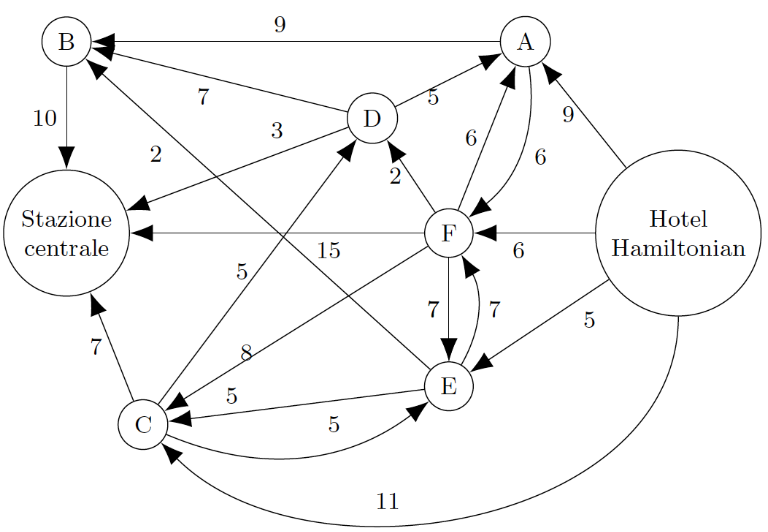
\includegraphics[width=12cm]{images/esercitazione/programmazione-lineare-mista/CorsaInStazione.png}
\end{center}

\paragraph{Svolgimento}

\begin{align*}
    min Z &= \Sigma _{(i,j) \in E} t_{ij} x_{ij} \\
    \Sigma _{z \mid (i,z) \in E} x_{iz} - \Sigma _{z \mid (z,i) \in E} x_{zi} &= 0 &\forall i \in V \setminus \{s,t\} \\
    \Sigma _{z \mid (s,z) \in E} x_{sz} - \Sigma _{z \mid (z,s) \in E} x_{zs} &= 1 \\
    \Sigma _{z \mid (t,z) \in E} x_{tz} - \Sigma _{z \mid (z,t) \in E} x_{zt} &= -1 \\
    x_{ij} &\in \{0,1\} &\forall i,j \in V
\end{align*}

\section{Colonnine di Ricarica}

\paragraph{Svolgimento}

dichiaro la funzione $V : Q \times Q \rightarrow \{1,0\}$ \\
che descrive con $V(q_x, q_y)$ se $q_x$ e $q_y$ sono adiacenti.

\begin{align*}
    min Z &= \Sigma ^ {|Q|} _ {i=1} x_i \\
    \Sigma ^ {|Q|} _ {i=1} V(q_i, q_j) x_i &\geq 1 &\forall j \in [1, |Q|] \\
    \forall i \in [1,Q] &\rightarrow x_i \in \{1,0\}
\end{align*}

\section{Gita al Parco Divertimenti}

dichiaro la funzione $P : A \rightarrow N^{+}$ \\
che descrive con $P(a_x)$ il punteggio della relativa attrazione.

dichiaro la funzione $T : A \rightarrow N^{+}$ \\
che descrive con $T(a_x)$ il tempo di visita della relativa attrazione.

dichiaro la funzione $F : A \rightarrow \{1,0\}$ \\
che descrive con $F(a_x)$ se la relativa attrazione e' Adrenaline.

dichiaro la funzione $G : A \rightarrow \{1,0\}$ \\
che descrive con $F(a_x)$ se la relativa attrazione e' Fantasy.

\begin{align*}
    max Z &= \Sigma ^ {|A|} _ {i=1} P(a_i) * x_i \\
    \Sigma ^ {|A|} _ {i=1} T(a_i) * x_i &\leq 540 \\
    \Sigma ^ {|A|} _ {i=1} F(a_i) * x_i &\geq 3 \\
    \Sigma ^ {|A|} _ {i=1} G(a_i) * x_i &\leq 1 \\
    x_{11} &\leq x_1 \\
    x_i &\leq 1 - x_5 &\forall i \in [1,|A|] \land F(x_i)\\
    \forall i \in [1,A] &\rightarrow x_i \in \{1,0\}
\end{align*}

